\documentclass[conference]{IEEEtran}

\usepackage[utf8]{inputenc}
\usepackage[english]{babel}
\usepackage{graphicx}

\begin{document}

\title{Implementing 'Gordon': A NAO Robot Receptionist to Enhance Efficiency in Critical Services Using Choregraphe and Python}

\author{
\IEEEauthorblockN{
        Diana Milligan\IEEEauthorrefmark{1},
        Filip Hanuš\IEEEauthorrefmark{1},
        Harry Williams\IEEEauthorrefmark{1},\\
        Jack Thompson\IEEEauthorrefmark{1},
        Natalie Leung\IEEEauthorrefmark{1}
}
\IEEEauthorblockA{
        \IEEEauthorrefmark{1}School of Engineering, College of Art, Technology and Environment,\\ University of the West of England, Bristol, UK\\
        Email: \{diana2.milligan, filip2.hanus, harry4.williams, jack2.ould, wing7.leung\}@live.uwe.ac.uk}
}

\maketitle

\begin{abstract}

This paper presents what is in this abstract. 

\end{abstract}

\begin{IEEEkeywords}

NAO Robot, Human Robot Interaction.

\end{IEEEkeywords}

\section{Introduction}

The purpose of this project is to use a Nao robotic platform to effectively perform a task that requires direct interaction with human. 
There are many different metrics that can be used to quantify the success of such a system, but as a broader definition an effective system 
should be able to receive and convey relevant information to an untrained user to achieve a wider goal.

A task that lends itself to this project brief is a reception environment, particularly in a medical setting. According to 
Mallorie \cite{mallorie2024}, managerial staff shortages within the NHS has pushed clinical staff to spend more time on administrative task over 
patient-facing care. To effectively reduce staffing requirements and thus make the running of medical centres less resource intensive, robotic 
systems can be integrated to alleviate the bulk of repetitive tasks. A good low-risk opportunity for this kind of integration is within a 
receptionist role where any possible errors are of a significantly lower severity than other roles (e.g. medical diagnosis and treatment).
A study conducted by Sutherland et al. \cite{Sutherland2019} tested the concept of a robotic receptionist for medical purposes, concluding that the robot displayed a 
"proffesional level of friendliness" that made it suited the role. However, the testing used a Wizard-of-Oz method with the robot only 
used as the interface between a user and a remote operator. Had all the behaviours been generated by the robot, there could have been 
a significant difference in how it was perceived by users.

Methods to create a sense of authority for robots has been explored through many different ways, many of which can be implemented within 
this project. Rae et al. \cite{Rae2013} explored the effect of height on robotic telepresence systems, concluding that a shorter "leader" was less persuasive 
for a the human follower. As well as the robot's stature, Rossi (need citation) found that contextual information such as the location of an interaction 
helped users infer the robot’s role.

Appearance has been argued to be a less important factor by Natarajan and Gombolay (need citation) who tested a variety of different variables for artificial agents, with 
behaviour being " the most significant factors in predicting the trust and compliance with the robot" rather 
than physical appearance. A Nao platform has been used by Cormier et al. \cite{cormier2013} to test the limitations of such compliance, finding that users would 
refuse to follow challenging orders from a robot if factors such as perceived intelligence or professionalism were compromised.


\section{Literature Review}

TBD

\section{Design and Methodology}

Our NAO-based receptionist system was designed with two main objectives:
\begin{enumerate}
        \item Streamlining patient check-in and
        \item Maintaining user trust and engagement.
\end{enumerate}

\begin{figure*}
        \centering
        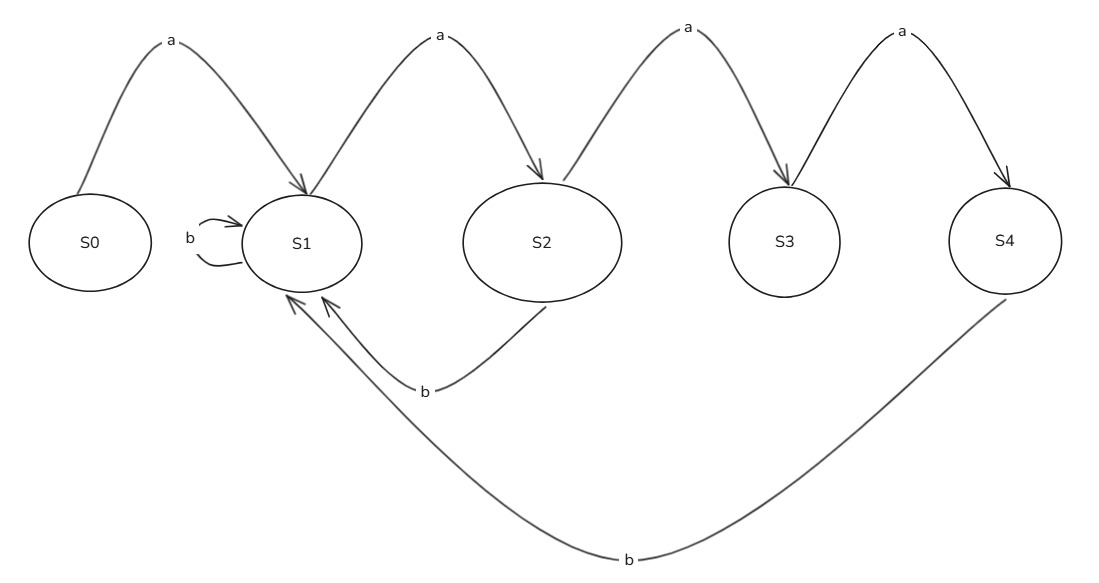
\includegraphics[width=.6\linewidth]{states.jpg}
        \caption{Different States and their Connections}
        \label{Different states}
\end{figure*}

\subsection{Overview of System States} Figure~\ref{Different states} illustrates our finite state machine, implemented
using Aldebaran’s Choregraphe and Python scripts:

\begin{enumerate} \item \textbf{Face Detection (State 0):} NAO continuously scans for faces. If a recognised face is detected, it waits for user input. This ensures worker's face(s) are stored in the form of initialisation.
        \item \textbf{Wave Detection (State 1):} A Mediapipe-based script running in Python identifies a waving hand signal. Upon detection, the system transitions to direct interaction mode.
        \item \textbf{Check-in Interaction (State 2):} NAO initiates a spoken dialogue to ask for appointment details. It uses inbuilt speech recognition configured for British English.
        \item \textbf{Email Notification (State 3):} On successful check-in, NAO sends an automated email to the relevant staff member. To circumvent network restrictions on SMTP, local testing used a laptop-based hotspot, with a fallback plan of staff intervention.
        \item \textbf{Feedback Collection (State 4):} NAO requests a brief rating from the user, storing any comments for later review.
\end{enumerate}

\subsection{Hardware and Software Setup} We ran Choregraphe on a laptop that communicates with the NAO robot over Wi-Fi.
For gestures, a laptop-mounted camera and a Python-based Mediapipe module detect and interpret waving motions.
Whenever network blocks occurred (e.g.\ institutional firewalls), we redirected connections through a personal hotspot to ensure uninterrupted email functionality.

\subsection{Design Rationale} We opted for a height-aligned placement of NAO to improve authority and user engagement,
as recommended by Rae et al.\cite{Rae2013}. This also aligns with Sutherland et al.\cite{Sutherland2019}, who showed the benefits of
a robotic receptionist in clinical settings. Our approach expands on their Wizard-of-Oz study by allowing NAO to generate all behaviours without remote operators.

\subsection{Contingency Measures} In practice, user trust decreases sharply when robots show consistent errors, as reported by Bistolfi~\cite{Bistolfi2022}.
Therefore, we embedded clear fallback steps:
\begin{itemize}
        \item If the reservation checkin fails, staff are alerted via an email.
\end{itemize}


\section{Testing and Results}

TBD

\section{Future Work}Facial recognition was planned and developed but was not able to be featured in the final testing due to 
technical difficulties. Future work on this project would include and expand upon this capability as recognising (and potentially 
analysing) individuals vastly increases the functionality and perceived intelligence of the system.

To improve the quality of the current conversations, integrating a more robust NLP algorithm increases the likelihood that the Nao 
robot correctly understands the user’s intent from a single output. Currently, any output outside of expected values is considered 
an error and handled accordingly. NLP allows more unexpected inputs to be parsed for key information that otherwise would’ve been 
missed, directing the robot towards a more appropriate response.

While these improvements would improve the technology, extensive user testing (especially within the intended medical space) is the 
best way to understand the system's shortcomings and improve accordingly.


\section{Conclusion}

TBD

\bibliographystyle{plain}
\bibliography{references}

\end{document}